\documentclass{standalone}
\usepackage{tikz}
\usetikzlibrary{patterns, positioning}


\begin{document}
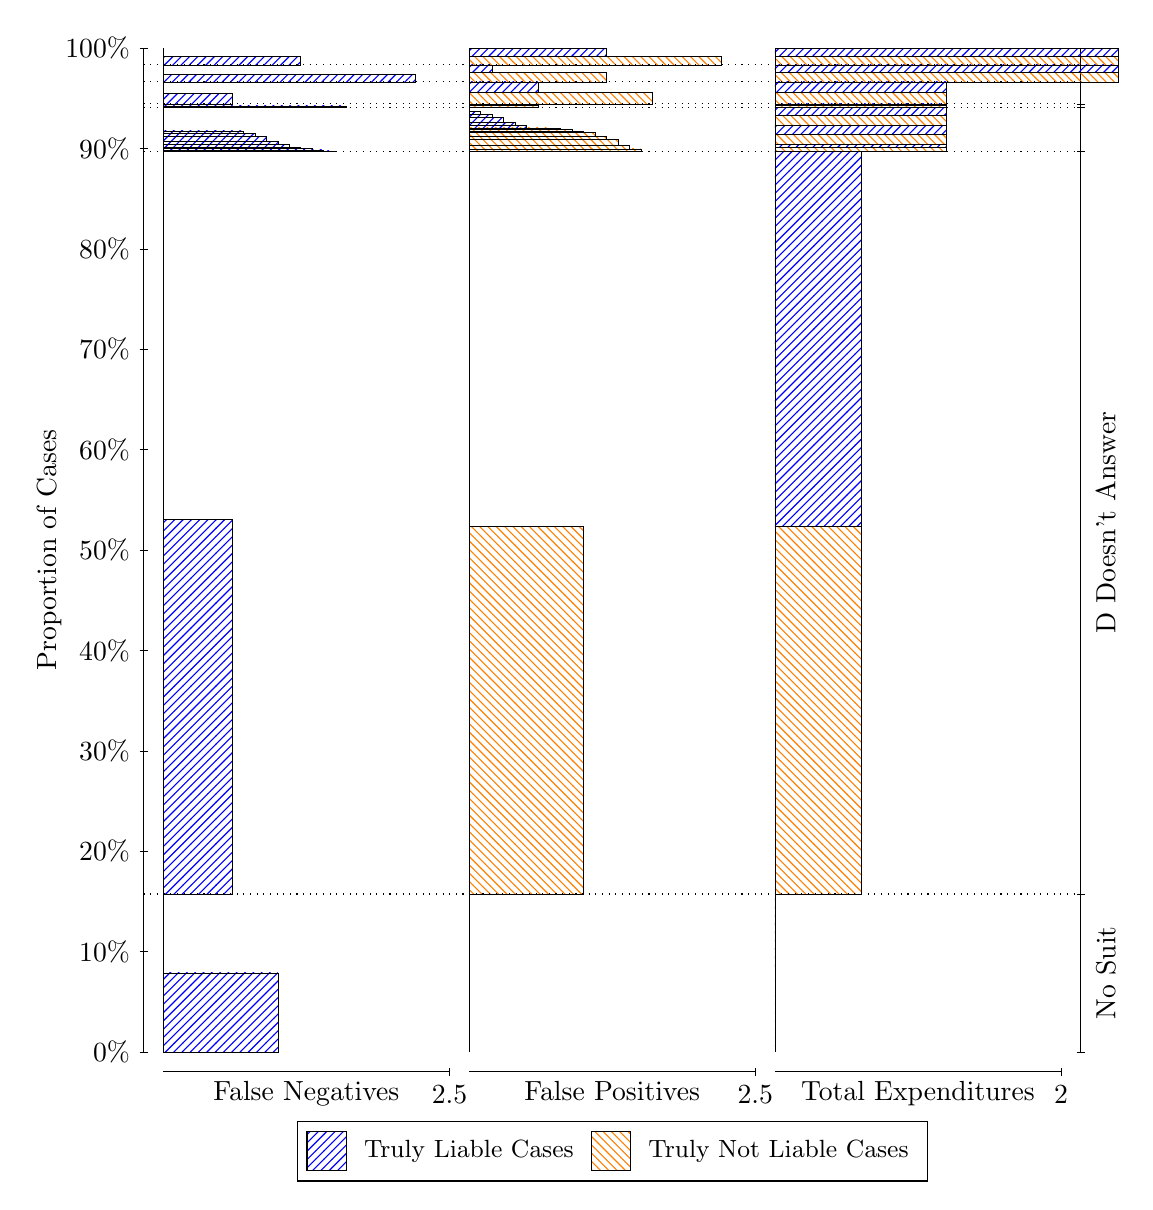
\begin{tikzpicture}
\draw[black, very thin] (1.5,1.75) -- (1.5,14.5);
\node[rotate=90, text=black, anchor=center] at (0.3, 8.125) {Proportion of Cases};
\draw[black, very thin] (1.45,1.75) -- (1.55,1.75);
\node[text=black, anchor=east] at (1.45, 1.75) {0\%};
\draw[black, very thin] (1.45,3.025) -- (1.55,3.025);
\node[text=black, anchor=east] at (1.45, 3.025) {10\%};
\draw[black, very thin] (1.45,4.3) -- (1.55,4.3);
\node[text=black, anchor=east] at (1.45, 4.3) {20\%};
\draw[black, very thin] (1.45,5.575) -- (1.55,5.575);
\node[text=black, anchor=east] at (1.45, 5.575) {30\%};
\draw[black, very thin] (1.45,6.85) -- (1.55,6.85);
\node[text=black, anchor=east] at (1.45, 6.85) {40\%};
\draw[black, very thin] (1.45,8.125) -- (1.55,8.125);
\node[text=black, anchor=east] at (1.45, 8.125) {50\%};
\draw[black, very thin] (1.45,9.4) -- (1.55,9.4);
\node[text=black, anchor=east] at (1.45, 9.4) {60\%};
\draw[black, very thin] (1.45,10.675) -- (1.55,10.675);
\node[text=black, anchor=east] at (1.45, 10.675) {70\%};
\draw[black, very thin] (1.45,11.95) -- (1.55,11.95);
\node[text=black, anchor=east] at (1.45, 11.95) {80\%};
\draw[black, very thin] (1.45,13.225) -- (1.55,13.225);
\node[text=black, anchor=east] at (1.45, 13.225) {90\%};
\draw[black, very thin] (1.45,14.5) -- (1.55,14.5);
\node[text=black, anchor=east] at (1.45, 14.5) {100\%};

\draw[black, very thin] (13.4,1.75) -- (13.4,14.5);
\draw[black, very thin] (13.35,1.75) -- (13.45,1.75);
\node[anchor=west] at (13.35, 1.75) {};
\draw[black, very thin] (13.35,3.7569) -- (13.45,3.7569);
\node[anchor=west] at (13.35, 3.7569) {};
\draw[black, very thin] (13.35,13.189) -- (13.45,13.189);
\node[anchor=west] at (13.35, 13.189) {};
\draw[black, very thin] (13.35,13.745) -- (13.45,13.745);
\node[anchor=west] at (13.35, 13.745) {};
\draw[black, very thin] (13.35,13.79) -- (13.45,13.79);
\node[anchor=west] at (13.35, 13.79) {};
\draw[black, very thin] (13.35,14.07) -- (13.45,14.07);
\node[anchor=west] at (13.35, 14.07) {};
\draw[black, very thin] (13.35,14.287) -- (13.45,14.287);
\node[anchor=west] at (13.35, 14.287) {};
\draw[black, very thin] (13.35,14.5) -- (13.45,14.5);
\node[anchor=west] at (13.35, 14.5) {};

\draw[black, very thin, pattern color=blue, pattern=north east lines] (1.75,1.75) rectangle (3.2033,2.7535);
\draw[black, very thin, pattern color=orange, pattern=north west lines] (1.75,2.7535) rectangle (1.75,3.7569);
\draw[black, very thin, pattern color=blue, pattern=north east lines] (1.75,3.7569) rectangle (2.622,8.5169);
\draw[black, very thin, pattern color=orange, pattern=north west lines] (1.75,8.5169) rectangle (1.75,13.189);
\draw[black, very thin, pattern color=blue, pattern=north east lines] (1.75,13.189) rectangle (3.93,13.195);
\draw[black, very thin, pattern color=blue, pattern=north east lines] (1.75,13.195) rectangle (3.7847,13.206);
\draw[black, very thin, pattern color=blue, pattern=north east lines] (1.75,13.206) rectangle (3.6393,13.225);
\draw[black, very thin, pattern color=blue, pattern=north east lines] (1.75,13.225) rectangle (3.494,13.238);
\draw[black, very thin, pattern color=blue, pattern=north east lines] (1.75,13.238) rectangle (3.3487,13.28);
\draw[black, very thin, pattern color=blue, pattern=north east lines] (1.75,13.28) rectangle (3.2033,13.315);
\draw[black, very thin, pattern color=blue, pattern=north east lines] (1.75,13.315) rectangle (3.058,13.381);
\draw[black, very thin, pattern color=blue, pattern=north east lines] (1.75,13.381) rectangle (2.9127,13.419);
\draw[black, very thin, pattern color=blue, pattern=north east lines] (1.75,13.419) rectangle (2.7673,13.447);
\draw[black, very thin, pattern color=orange, pattern=north west lines] (1.75,13.447) rectangle (1.75,13.745);
\draw[black, very thin, pattern color=blue, pattern=north east lines] (1.75,13.745) rectangle (4.0753,13.766);
\draw[black, very thin, pattern color=orange, pattern=north west lines] (1.75,13.766) rectangle (1.75,13.79);
\draw[black, very thin, pattern color=blue, pattern=north east lines] (1.75,13.79) rectangle (2.622,13.921);
\draw[black, very thin, pattern color=orange, pattern=north west lines] (1.75,13.921) rectangle (1.75,14.07);
\draw[black, very thin, pattern color=blue, pattern=north east lines] (1.75,14.07) rectangle (4.9473,14.163);
\draw[black, very thin, pattern color=orange, pattern=north west lines] (1.75,14.163) rectangle (1.75,14.287);
\draw[black, very thin, pattern color=blue, pattern=north east lines] (1.75,14.287) rectangle (3.494,14.395);
\draw[black, very thin, pattern color=orange, pattern=north west lines] (1.75,14.395) rectangle (1.75,14.5);
\draw[black, very thin, pattern color=orange, pattern=north west lines] (5.6333,1.75) rectangle (5.6333,2.7535);
\draw[black, very thin, pattern color=blue, pattern=north east lines] (5.6333,2.7535) rectangle (5.6333,3.7569);
\draw[black, very thin, pattern color=orange, pattern=north west lines] (5.6333,3.7569) rectangle (7.0867,8.4288);
\draw[black, very thin, pattern color=blue, pattern=north east lines] (5.6333,8.4288) rectangle (5.6333,13.189);
\draw[black, very thin, pattern color=orange, pattern=north west lines] (5.6333,13.189) rectangle (7.8133,13.22);
\draw[black, very thin, pattern color=orange, pattern=north west lines] (5.6333,13.22) rectangle (7.668,13.265);
\draw[black, very thin, pattern color=orange, pattern=north west lines] (5.6333,13.265) rectangle (7.5227,13.341);
\draw[black, very thin, pattern color=orange, pattern=north west lines] (5.6333,13.341) rectangle (7.3773,13.381);
\draw[black, very thin, pattern color=orange, pattern=north west lines] (5.6333,13.381) rectangle (7.232,13.429);
\draw[black, very thin, pattern color=orange, pattern=north west lines] (5.6333,13.429) rectangle (7.0867,13.445);
\draw[black, very thin, pattern color=orange, pattern=north west lines] (5.6333,13.445) rectangle (6.9413,13.466);
\draw[black, very thin, pattern color=orange, pattern=north west lines] (5.6333,13.466) rectangle (6.796,13.478);
\draw[black, very thin, pattern color=orange, pattern=north west lines] (5.6333,13.478) rectangle (6.6507,13.486);
\draw[black, very thin, pattern color=blue, pattern=north east lines] (5.6333,13.486) rectangle (6.36,13.515);
\draw[black, very thin, pattern color=blue, pattern=north east lines] (5.6333,13.515) rectangle (6.2147,13.552);
\draw[black, very thin, pattern color=blue, pattern=north east lines] (5.6333,13.552) rectangle (6.0693,13.618);
\draw[black, very thin, pattern color=blue, pattern=north east lines] (5.6333,13.618) rectangle (5.924,13.653);
\draw[black, very thin, pattern color=blue, pattern=north east lines] (5.6333,13.653) rectangle (5.7787,13.695);
\draw[black, very thin, pattern color=blue, pattern=north east lines] (5.6333,13.695) rectangle (5.6333,13.745);
\draw[black, very thin, pattern color=orange, pattern=north west lines] (5.6333,13.745) rectangle (6.5053,13.769);
\draw[black, very thin, pattern color=blue, pattern=north east lines] (5.6333,13.769) rectangle (5.6333,13.79);
\draw[black, very thin, pattern color=orange, pattern=north west lines] (5.6333,13.79) rectangle (7.9587,13.939);
\draw[black, very thin, pattern color=blue, pattern=north east lines] (5.6333,13.939) rectangle (6.5053,14.07);
\draw[black, very thin, pattern color=orange, pattern=north west lines] (5.6333,14.07) rectangle (7.3773,14.194);
\draw[black, very thin, pattern color=blue, pattern=north east lines] (5.6333,14.194) rectangle (5.924,14.287);
\draw[black, very thin, pattern color=orange, pattern=north west lines] (5.6333,14.287) rectangle (8.8307,14.392);
\draw[black, very thin, pattern color=blue, pattern=north east lines] (5.6333,14.392) rectangle (7.3773,14.5);
\draw[black, very thin, pattern color=orange, pattern=north west lines] (9.5167,1.75) rectangle (9.5167,2.7535);
\draw[black, very thin, pattern color=blue, pattern=north east lines] (9.5167,2.7535) rectangle (9.5167,3.7569);
\draw[black, very thin, pattern color=orange, pattern=north west lines] (9.5167,3.7569) rectangle (10.607,8.4288);
\draw[black, very thin, pattern color=blue, pattern=north east lines] (9.5167,8.4288) rectangle (10.607,13.189);
\draw[black, very thin, pattern color=orange, pattern=north west lines] (9.5167,13.189) rectangle (11.697,13.237);
\draw[black, very thin, pattern color=blue, pattern=north east lines] (9.5167,13.237) rectangle (11.697,13.279);
\draw[black, very thin, pattern color=orange, pattern=north west lines] (9.5167,13.279) rectangle (11.697,13.407);
\draw[black, very thin, pattern color=blue, pattern=north east lines] (9.5167,13.407) rectangle (11.697,13.52);
\draw[black, very thin, pattern color=orange, pattern=north west lines] (9.5167,13.52) rectangle (11.697,13.641);
\draw[black, very thin, pattern color=blue, pattern=north east lines] (9.5167,13.641) rectangle (11.697,13.745);
\draw[black, very thin, pattern color=orange, pattern=north west lines] (9.5167,13.745) rectangle (11.697,13.769);
\draw[black, very thin, pattern color=blue, pattern=north east lines] (9.5167,13.769) rectangle (11.697,13.79);
\draw[black, very thin, pattern color=orange, pattern=north west lines] (9.5167,13.79) rectangle (11.697,13.939);
\draw[black, very thin, pattern color=blue, pattern=north east lines] (9.5167,13.939) rectangle (11.697,14.07);
\draw[black, very thin, pattern color=orange, pattern=north west lines] (9.5167,14.07) rectangle (13.877,14.194);
\draw[black, very thin, pattern color=blue, pattern=north east lines] (9.5167,14.194) rectangle (13.877,14.287);
\draw[black, very thin, pattern color=orange, pattern=north west lines] (9.5167,14.287) rectangle (13.877,14.392);
\draw[black, very thin, pattern color=blue, pattern=north east lines] (9.5167,14.392) rectangle (13.877,14.5);
\draw[black, dotted] (1.5,3.7569) -- (13.4,3.7569);
\draw[black, dotted] (1.5,13.189) -- (13.4,13.189);
\draw[black, dotted] (1.5,13.745) -- (13.4,13.745);
\draw[black, dotted] (1.5,13.79) -- (13.4,13.79);
\draw[black, dotted] (1.5,14.07) -- (13.4,14.07);
\draw[black, dotted] (1.5,14.287) -- (13.4,14.287);
\draw[black, very thin] (1.75,1.5) -- (5.3833,1.5);
\node[text=black, anchor=north] at (3.5667, 1.5) {False Negatives};
\draw[black, very thin] (5.3833,1.45) -- (5.3833,1.55);
\node[text=black, anchor=north] at (5.3833, 1.45) {2.5};

\draw[black, very thin] (5.6333,1.5) -- (9.2667,1.5);
\node[text=black, anchor=north] at (7.45, 1.5) {False Positives};
\draw[black, very thin] (9.2667,1.45) -- (9.2667,1.55);
\node[text=black, anchor=north] at (9.2667, 1.45) {2.5};

\draw[black, very thin] (9.5167,1.5) -- (13.15,1.5);
\node[text=black, anchor=north] at (11.333, 1.5) {Total Expenditures};
\draw[black, very thin] (13.15,1.45) -- (13.15,1.55);
\node[text=black, anchor=north] at (13.15, 1.45) {2};

\node[text=black, centered, rotate=90] at (13.72, 2.7535) {No Suit};
\node[text=black, centered, rotate=90] at (13.72, 8.4729) {D Doesn't Answer};






\draw (7.449999999999999,1.5) node[draw=none] (baseCoordinate) {};
\begin{scope}[align=center]
        \matrix[scale=0.5, draw=black, below=0.5cm of baseCoordinate, nodes={draw}, column sep=0.1cm]{
            \node[rectangle, draw, minimum width=0.5cm, minimum height=0.5cm, pattern color=blue, pattern=north east lines] {}; &
            \node[draw=none, font=\small, text=black] (B) {Truly Liable Cases}; &
            \node[rectangle, draw, minimum width=0.5cm, minimum height=0.5cm, pattern color=orange, pattern=north west lines] {}; &
            \node[draw=none, font=\small, text=black] (B) {Truly Not Liable Cases}; \\
            };
\end{scope}

\end{tikzpicture}
\end{document}